%Når afsnit 3 er færdig, så ved læseren hvad man skal gøre.
In our compilation from Hermes to ARM64 using Moscow ML\footnote{Moscow ML is a functional programming language widely used for teaching and research. More can be found at \url{http://www.itu.dk/~sestoft/mosml.html}}, we need to be aware of several things..
We are skipping some steps, as the current implementation is from Hermes to C and then to ARM.
But by skipping these steps, we have an easier time analyzing and optimizing. The question is how do we do it and what do we need to consider?

\section{}
%Afsnit 3 analyserer vi problemet (oversættelsen fra Hermes uden sidekanaler til ARM). Hvordan gør vi det egentlig, hvad skal vi være opmærksom på. Vækrtøjer vi bruger, hvorfor bruger vi dem, hvad skal vi gøre for at de kan bruges.
The first step is to compile Hermes into RSSA. We use the procedure introduced in section \ref{section - RIL}.
We can do this in two runs: first we translate into RIL, and then we translate into RSSA.
The reason for doing it in two steps is to postpone the problem of register allocation, and keep the two problems seperated.
We will be creating an abstract syntax tree that RIL and RSSA will share.
As seen in figure ~\ref{fig:RIL vs RSSA}, the main difference between the two representations is the subscript index on the left-values.
\begin{figure}[htp]
  \begin{center}
    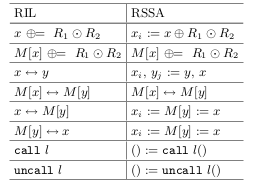
\includegraphics[width=0.6\textwidth]{RIL_RSSA_syntax.png}
  \end{center}
  \caption[caption]{RIL and RSSA syntax from\cite{10.1007/978-3-319-41579-6_16}}
  \label{fig:RIL vs RSSA}
\end{figure} \\
%\begin{wrapfigure}{r}{0.60\textwidth}
%  \begin{center}
%    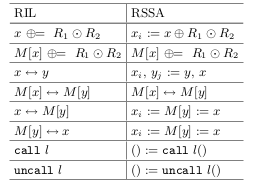
\includegraphics[width=0.55\textwidth]{RIL_RSSA_syntax.png}
%  \end{center}
%  \caption[caption]{RIL and RSSA syntax from\cite{10.1007/978-3-319-41579-6_16}}
%  \label{fig: RIL vs RSSA}
%\end{wrapfigure} \\
Variables that are going to have an index can be represented in SML as a tuple of a string variable name and an integer option index. The integer option can be NONE in the first iteration to RIL, and SOME int in the second iteration to RSSA. This makes it easy to seperate the two tasks and handle the indexing once the program has already been transformed to RIL.

\section{Protecting versus side-channels}
%Oplagt at have et afsnit der beskriver de dele af ARM der er relevant i forhold til oversættelsen. Finder de instruktioner der er relevant. Hvad skal vi være opmærksomme på. Er der nogle vi ikke kan bruge fordi de generer sidekanaler?

\subsection{Grammar}
The grammar of Hermes is as follows:
% TODO: Skriv bedre
I've made some changes to the grammar. I've added const array decl
\begin{figure}[htp]
\centering
\begin{tabular}{>{$}l<{$}>{$}r<{$}>{$}l<{$}}
    Program   & \rightarrow & Procedure^+ \\[7pt]
    Procedure & \rightarrow & \textbf{id} \; ( \; Decls2^? \; ) \; Stmt \\[7pt]
    Stmt      & \rightarrow &; \\
              & |           & Lval \; \textbf{update} \; Exp \;; \\
              & |           & Lval\text{++} \;; \\
              & |           & Lval\text{- -} \;; \\
              & |           & \texttt{if} \; ( \; Exp \; ) \; Lval \; \textbf{update} \; Exp \;; \\
              & |           & Lval \; \text{<->} \; Lval \;; \\
              & |           & \texttt{if} \; ( \; Exp \; ) \; Lval \; \text{<->} \; Exp \;; \\
              & |           & \texttt{for} \; ( \; \textbf{id} = Exp \; ; \; Exp \; ) \; Stmt  \;; \\
              & |           & \texttt{assert} \; ( \; Exp \; ) \;; \\
              & |           & \texttt{call} \; \textbf{id} \; ( \; Lvals \; ) \;; \\
              & |           & \texttt{uncall} \; \textbf{id} \; ( \; Lvals \; ) \;; \\
              & |           & \texttt{printf} \; ( \; \textbf{stringConst} \; , \; Lvals \; ) \;; \\
              & |           & \texttt{scanf} \; ( \; \textbf{stringConst} \; , \; Lvals \; ) \;; \\
              & |           & \{ \; Decls1 \; Stmt^* \; \} \\[7pt]
    Exp       & \rightarrow & Lval \\
              & |           & \textbf{numConst} \; \\
              & |           & Exp \; \textbf{binOp} \; Exp \\
              & |           & \textbf{unOp} \; Exp \\
              & |           & ( \; Exp \; ) \; \\[7pt]
    Lval      & \rightarrow & \textbf{id}\\
              & |           & \textbf{id} \; [ \; Exp \; ] \\[7pt]
    Lvals     & \rightarrow & Lval \\
              & |           & Lval \; , \; Lvals \\[7pt]
    VarSpec   & \rightarrow & \textbf{id}\\
              & |           & \textbf{id} \; [ \; \textbf{numConst} \; ] \\[7pt]
    VarSpecs  & \rightarrow & VarSpec \\
              & |           & VarSpec \; , \; VarSpecs \\[7pt]
    Decls1    & \rightarrow & \\
              & |           & \textbf{type} \; Varspecs \; ; \; Decls1\\
              & |           & \texttt{const}\;\textbf{type}\;\textbf{id}\;=\textbf{numConst}\;;\;Decls1\;\\[7pt]
    Decls2    & \rightarrow & \textbf{type} \; VarSpec \\
              & |           &  \textbf{type} \; VarSpec \; , \; Decls2

\end{tabular}
\caption{Grammar of Hermes.}
\label{fig: grammar}
\end{figure}



\section{Translation by hand}
%I afsnit 3 kan man vise hvordan man oversætter et Hermes program til RIL (det vi gjorde i hånden). Skal hjælpe læseren med at forstå nogle af de mere abstrakte begreber.
